\chapter{Methods} \label{chap:methods}
Methods intro text...

\section{Network Pruning} \label{sec:network_pruning}
Network pruning text...

Network Shrinking...

\section{Feature Selection} \label{sec:feature_selection}
Minimal network structure text...

Pathing in Net (Feature Selection)

Feature Energy computation

\section{Network Visualization} \label{sec:network_visualization}
Graphical user interface text...

\newpage
\section{Speech Data Gathering} \label{sec:speech_data_gathering}
The presented methods are tested on several examples (\cref{chap:examples}) and one of them rests in classification of phonemes. By definition a phoneme is one of the units of sound that distinguish one word from another in a particular language \citep{wiki:mnist}. We focus on Czech language and consider $ 40 $ phonemes listed in \cref{tab:methods:phonetic_alphabet}. This section describes the way of gathering such phonemes and building a dataset for classification.

\begin{table}[H]
\centering
\scalebox{0.8}{
\begin{tabular}{|c|c|c||c|c|c||c|c|c|}
\hline
\textit{sound} & \textit{phoneme} & \textit{example} & \textit{sound} & \textit{phoneme} & \textit{example} & \textit{sound} & \textit{phoneme} & \textit{example} \\ \hline \hline
a  & a                & mám\textbf{a}             & ch & x                & \textbf{ch}yba            & ř     & R                & mo\textbf{ř}e             \\ \hline
á  & A                & t\textbf{á}ta             & i  & i                & p\textbf{i}vo             & ř     & Q                & t\textbf{ř}i              \\ \hline
au & Y                & \textbf{au}to             & í  & I                & v\textbf{í}no             & s     & s                & o\textbf{s}el             \\ \hline
b  & b                & \textbf{b}od              & j  & j                & vo\textbf{j}ák            & š     & S                & po\textbf{š}ta            \\ \hline
c  & c                & o\textbf{c}el             & k  & k                & o\textbf{k}o              & t     & t                & o\textbf{t}ec             \\ \hline
č  & C                & o\textbf{č}i              & l  & l                & \textbf{l}oď              & ť     & T                & ku\textbf{t}il            \\ \hline
d  & d                & \textbf{d}ům              & m  & m                & \textbf{m}ír              & u     & u                & r\textbf{u}m              \\ \hline
ď  & D                & \textbf{d}ěti             & n  & n                & \textbf{n}os              & ú (ů) & U                & r\textbf{ů}že             \\ \hline
e  & e                & p\textbf{e}s              & n  & N                & ba\textbf{n}ka            & v     & v                & \textbf{v}lak             \\ \hline
é  & E                & l\textbf{é}pe             & ň  & J                & la\textbf{ň}              & z     & z                & ko\textbf{z}a             \\ \hline
eu & F                & \textbf{eu}nuch           & o  & o                & b\textbf{o}k              & ž     & Z                & \textbf{ž}ena             \\ \hline
f  & f                & \textbf{f}acka            & ou & y                & p\textbf{ou}to            &       & \_sil\_          & (silence)                 \\ \hline
g  & g                & \textbf{g}uma             & p  & p                & \textbf{p}rak             &       &                  &                           \\ \hline
h  & h                & \textbf{h}ad              & r  & r                & \textbf{r}ak              &       &                  &                           \\ \hline
\end{tabular}}
\caption{Czech phonetic alphabet.}
\label{tab:methods:phonetic_alphabet}
\end{table}

The generation of a speech dataset consists of the following steps, where the work done in steps $ 1-3 $ is taken over from \citep{smidl_pc}.

\begin{enumerate}
\item acquisition of real voice recordings;
\item feature extraction from the sound signals (parameterization);
\item labeling the data;
\item definition of one sample;
\item splitting samples into training/development/testing sets.
\end{enumerate}

\subsection*{Acquisition of Voice Recordings}
The phoneme dataset is made of real speech recordings from a car interior environment, provided by (Škoda, ?? ref). We are talking about simple voice instructions for a mobile phone or a navigation system, many of them are names of people, streets or towns only. In total $ 14523 $ recordings (\texttt{.wav} files) of various length (and so number of phonemes) were obtained.

\subsection*{Parameterization}
The goal of parameterization is to represent each recording by a vector of features. A commonly known procedure based on MFCCs is used. A nice detailed explanation of this method can be found e.g. in \citep{online:mfcc}. 

The idea behind MFCCs originates in the fact that a shape of human vocal tract (including tongue, teeth etc.) determines what sound comes out. The shape of the vocal tract manifests itself in the envelope of the short time power spectrum, and the job of MFCCs is to accurately represent this envelope.

The parameterization workflow is summarized by these steps:

\begin{enumerate}
\item \textit{splitting the signal into short frames};

\cref{fig:methods:mfcc_framing} illustrates how a sound signal is splitted into short frames. The parameters are
\begin{align*}
frame\_size &= 0.025 \,s \,= 25 \,ms \\
frame\_shift &= 0.01 \,s \,= 10 \,ms
\end{align*}
Using the sampling frequency $ f_s = 8 kHz $, we get frames of length $ 200 $.

\begin{figure}[H]
\centering
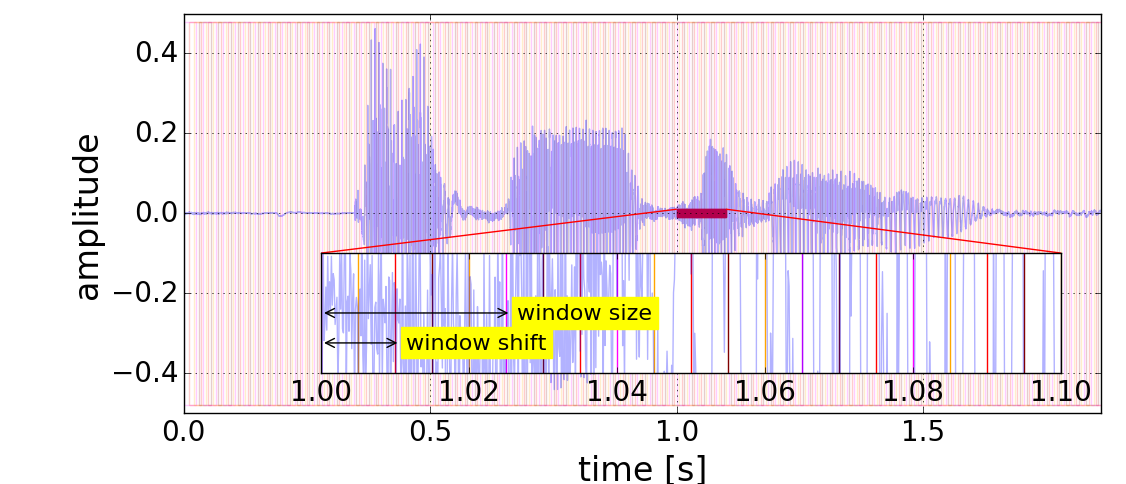
\includegraphics[width=\textwidth]{mfcc_framing.png}
\caption{Framing a sound signal.}
\label{fig:methods:mfcc_framing}
\end{figure}

We assume each frame captures one possible shape of the human vocal tract and therefore is capable of carrying one phoneme only. The next steps are applied for every single frame.

\item \textit{calculation of the periodogram estimate of the power spectrum}; 

The aim is to identify which frequencies are present. In order to do so, we apply the Hamming window and perform the discrete Fourier Transform (DFT; \cref{eq:dft}).

\begin{equation} \label{eq:dft}
S(k) = \displaystyle\sum_{n=0}^{N-1} s_n \cdot e^{-2 \pi i \frac{kn}{N}}, \qquad k = 0, ..., N-1
\end{equation}

, where $ N $ (in this case $ N = 200 $) is the signal length. Then we take the absolute value $ |S(k)| $.

\item \textit{application of the mel filterbank to the power spectra, summation of the energy in each filter, taking a logarithm of the result};

Next, we use a filterbank of triangle filters (illustrated in \cref{fig:methods:mfcc_filterbank}) predefined on the transmitted band ($ bw = \frac{f_s}{2} = 4kHz $) to get a single value per filter. We use $ 40 $ filters, therefore, each frame is now described by a vector of $ 40 $ numbers.

\begin{figure}[H]
\centering
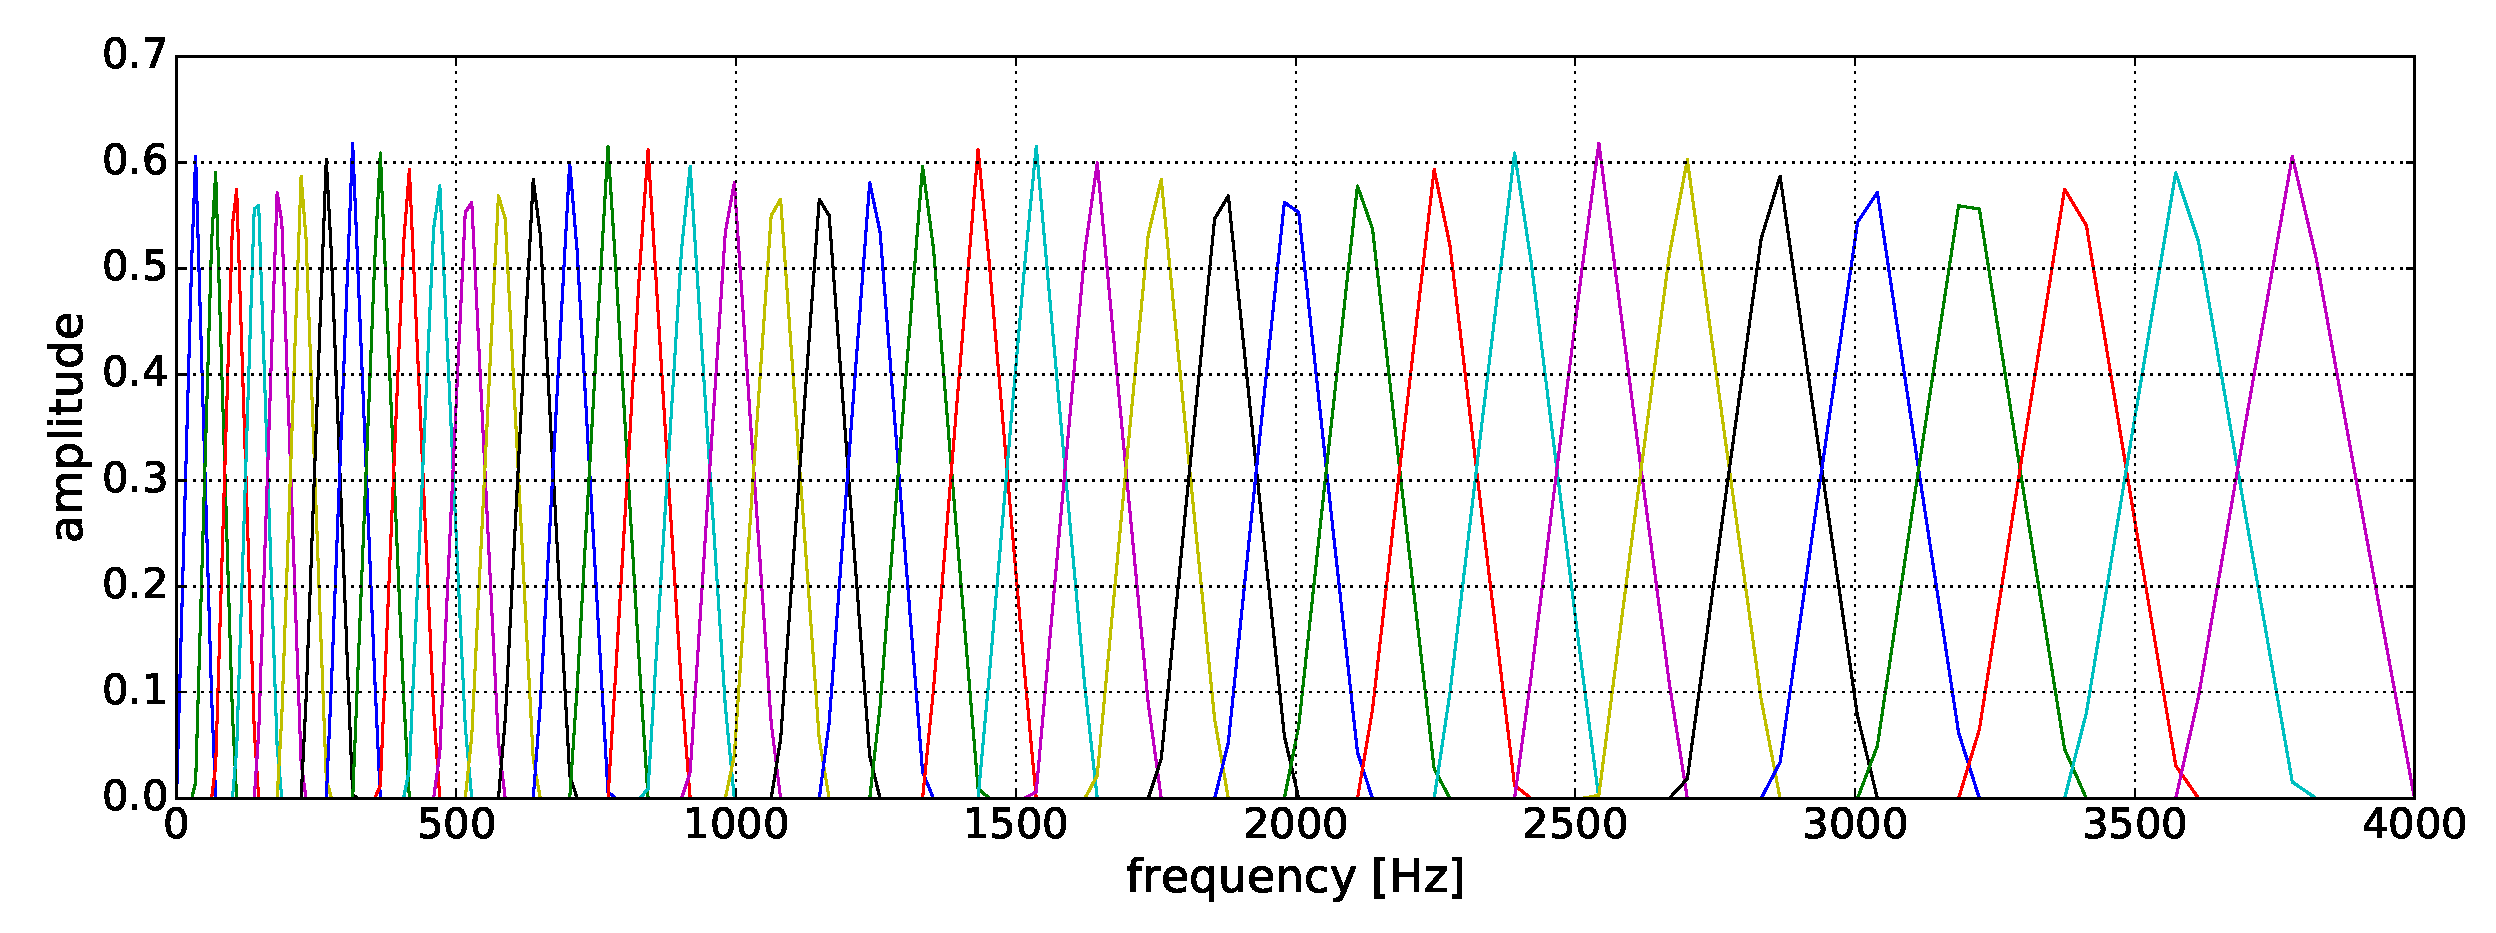
\includegraphics[width=\textwidth]{mfcc_filterbank}
\caption{Mel Filterbank of 40 filters in Hertz-axis.}
\label{fig:methods:mfcc_filterbank}
\end{figure}

Finally, a logarithm of the result is taken and considered as a description of the frame (phoneme). Usually, a discrete Cosine Transform (DCT) is applied at the end, however, it is not done in this work. The result of a signal parameterization is a matrix shown in \cref{eq:parameterization_result}.

\begin{equation} \label{eq:parameterization_result}
recording\_params = 
\begin{bmatrix}
    f_{11} & f_{12} & f_{13} & \dots  & f_{1F} \\
    f_{21} & f_{22} & f_{23} & \dots  & f_{2F} \\
    \vdots & \vdots & \vdots & \ddots & \vdots \\
    f_{W1} & f_{W2} & f_{W3} & \dots  & f_{WF}
\end{bmatrix}
\end{equation}

, where $ F = 40 $ is the number of filters and $ W $ is the number of frames (windows) depending on the duration of a recording. Value $ f_{12} $ then belongs to the feature computed with the second filter in the first frame.
\end{enumerate}

\subsection*{Data Labeling}
We perform a supervised learning method, hence the data must be labeled. To the so a speech recognition method based on Hidden Markov Models (HMMs) from \citep{smidl_pc} is used. It labels the frames of each recording as shown on an example in \cref{tab:methods:labeling_example}.

\begin{table}[H]
\centering
\begin{tabular}{|c|c|c|}
\hline
\multicolumn{3}{|c|}{recording\_name}                                                                                     \\ \hline
\multicolumn{1}{|l|}{\textit{frame\_in}} & \multicolumn{1}{l|}{\textit{frame\_out}} & \multicolumn{1}{l|}{\textit{phoneme}} \\ \hline
0                                       & 16                                      & \_sil\_                               \\ \hline
16                                      & 25                                      & a                                     \\ \hline
25                                      & 32                                      & n                                     \\ \hline
32                                      & 44                                      & o                                     \\ \hline
44                                      & 65                                      & \_sil\_                               \\ \hline
\end{tabular}
\caption{Example of labeled recording.}
\label{tab:methods:labeling_example}
\end{table}

It says that features extracted from this recording consist of $ 9 $ fourty-dimensional vectors representing phoneme \texttt{"a"}, $ 7 $ vectors of phoneme \texttt{"n"}, etc.

\subsection*{Forming a Sample}
The $ 40 $ phonemes listed in \cref{tab:methods:phonetic_alphabet} are naturally labels of classes, so we have a fourty-class classification problem. Having the information from previous section, one can match the extracted features with corresponding phonemes (classes). Now the task is to define the form of one sample.

\cref{fig:methods:sample_forming_bs} goes with the example in \cref{tab:methods:labeling_example}. The numbers in the first line are frame indices. The second line contains the known frame labels, where each frame is described by a vector of $ 40 $ features.

There is a possibility to take all frames labeled as \texttt{"a"} and consider the corresponding vectors directly as samples. However, as the labeling was not done manually and therefore cannot be considered as $ 100\% $ correct, we introduce a parameter called \texttt{border\textunderscore size}. \cref{fig:methods:sample_forming_bs} shows that we omit the frames on borders with another phoneme label and take only those in the middle.

\begin{figure}[H]
\centering
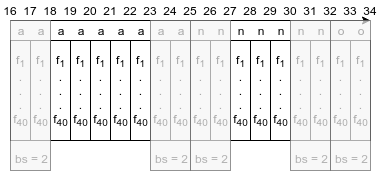
\includegraphics[width=0.8\textwidth]{sample_forming_bs}
\caption{Forming a sample, illustration of parameter \texttt{border\textunderscore size (bs)}.}
\label{fig:methods:sample_forming_bs}
\end{figure}

Moreover, in \cref{fig:methods:sample_forming_cs} parameter \texttt{context\textunderscore size} is introduced. The idea is to consider not only the information of one frame, but also of its context, into one sample.

\begin{figure}[H]
\centering
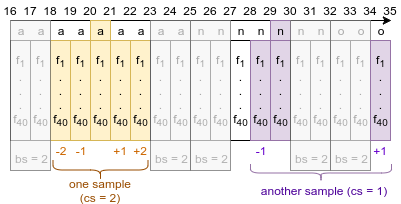
\includegraphics[width=0.75\textwidth]{sample_forming_cs}
\caption{Forming a sample, illustration of parameter \texttt{context\textunderscore size (cs)}.}
\label{fig:methods:sample_forming_cs}
\end{figure}

Based on the chosen context size $ cs $ the previous and subsequent vectors are added one by one and forms one feature vector of length $ 40 \cdot (2cs+1) $. An example for $ cs = 2 $ is illustrated in \cref{fig:methods:feature_vector}.

\begin{figure}[H]
\centering
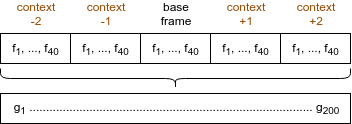
\includegraphics[width=0.8\textwidth]{feature_vector}
\caption{Example of building a feature vector with \texttt{context\textunderscore size} $ cs = 2 $.}
\label{fig:methods:feature_vector}
\end{figure}

Talking about \cref{fig:methods:feature_vector}, features $ g_1, g_2, ..., g_{200} $ gives the final feature vector of one sample, which takes the label of the base frame.

The last parameter of the speech dataset generation is the number of samples per class (\texttt{n\textunderscore samples}). The rule of thumb is the more samples the better training results, however, getting best possible training results is not the objective of this work. Therefore we often use less samples to speed up the training process.

To summarize this section, we end up with three parameters of the speech dataset generation process:

\begin{itemize}
\item \texttt{border\textunderscore size} (see \cref{fig:methods:sample_forming_bs})
\item \texttt{context\textunderscore size} (see \cref{fig:methods:sample_forming_cs})
\item \texttt{n\textunderscore samples} per class
\end{itemize}

\subsection*{Splitting data into three disjunctive sets}
\cref{fig:methods:three_sets} shows a general approach of data splitting in machine learning. It is used for all classification problems in this work. The training data is used to set up model parameters. Development data is then used for testing during the training process, in order to adjust some learning parameters based on the test results. Finally, a trained model is tested on never-seen testing data. We use splitting: $ 80\% $ training set; $ 10\% $ development set; $ 10\% $ testing set.

\begin{figure}[H]
\centering
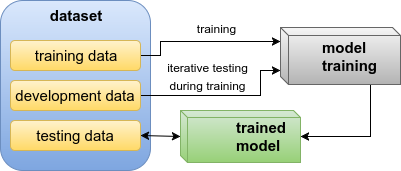
\includegraphics[width=0.7\textwidth]{three_sets}
\caption{Using three disjunctive sets of data for a general machine learning process.}
\label{fig:methods:three_sets}
\end{figure}